\documentclass[tikz]{standalone}

\begin{document}
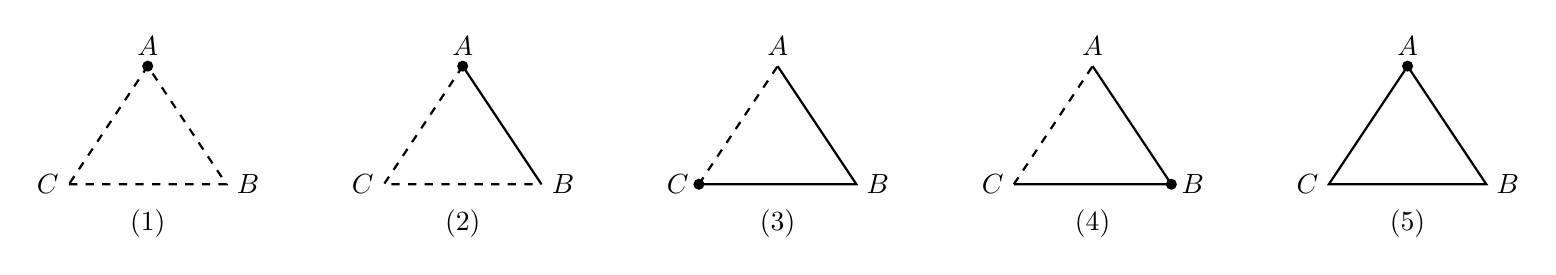
\begin{tikzpicture}[thick]
% Triangle with dashed edges
\draw[dashed] (0,0) node[left]{$C$} -- (2,0) node[right]{$B$} -- (1,1.5) node[above]{$A$} -- cycle;
\fill (1,1.5) circle (2pt);
\node at (1,-0.5) {(1)};

% Solid AB, dashed AC and highlighted node A
\draw (5,1.5) node[above]{$A$} -- (6,0) node[right]{$B$};
\draw[dashed] (5,1.5) -- (4,0) node[left]{$C$} -- (6,0);
\fill (5,1.5) circle (2pt);
\node at (5,-0.5) {(2)};

% Solid AB and BC, dashed AC and highlighted node C
\draw (8,0) node[left]{$C$} -- (10,0) node[right]{$B$} -- (9,1.5) node[above]{$A$};
\draw[dashed] (8,0) -- (9,1.5);
\fill (8,0) circle (2pt);
\node at (9,-0.5) {(3)};

% Solid AB and BC, dashed AC and highlighted node B
\draw (12,0) node[left]{$C$} -- (14,0) node[right]{$B$} -- (13,1.5) node[above]{$A$};
\draw[dashed] (12,0) -- (13,1.5);
\fill (14,0) circle (2pt);
\node at (13,-0.5) {(4)};

% Solid triangle with highlighted node A
\draw (16,0) node[left]{$C$} -- (18,0) node[right]{$B$} -- (17,1.5) node[above]{$A$} -- cycle;
\fill (17,1.5) circle (2pt);
\node at (17,-0.5) {(5)};

\end{tikzpicture}
\end{document}
